\section{Learning NFH}
\label{sec:learning}

In this section, we introduce $\lstar$-based learning algorithms for the fragments $\nfhf$ and 
$\nfhe$. 
We first survey the $\lstar$ algorithm \cite{Angluin87}, and then describe the relevant 
adjustments for our case.

\subsection{Angluin's $\lstar$ Algorithm}

$\lstar$ consists of two entities: a {\em learner}, who wishes to learn a DFA $A$ for an unknown (regular) language $\cal L$, and a {\em teacher}, who knows $\cal L$.
During the learning process, the learner asks the teacher two types of queries: {\em membership queries} (``is the word $w$ in $\cal L$?'') and {\em equivalence queries} (``is $A$ a DFA for $\cal L$?'').

The learner maintains $A$ in the form of an {\em observation table} $T$ of truth values, whose rows $D, D\cdot\Sigma$ and columns $E$ are sets of words over $\Sigma$, where $D$ is prefix-closed, and $E$ is suffix-closed. Initially, $D = E = \{\epsilon\}$. 
For a row $d$ and a column $e$, the entry for $T(d,e)$ is $\true$ iff $d\cdot e \in{\cal L}$. The entries are filled via membership queries.
The vector of truth values for row $d$ is denoted $\row(d)$. Intuitively, the rows in $D$ determine the states of $A$, and the rows in $D\cdot\Sigma$ determine the transitions of $A$: the state $\row(d\cdot\sigma)$ is reached from $\row(d)$ upon reading $\sigma$. 

The learner updates $T$ until it is {\em closed}, which, intuitively, ensures a full transition relation and {\em consistent}, which, intuitively, ensures a deterministic transition relation.
If $T$ is not closed or not consistent then more rows or more columns are added to $T$, respectively. 

\stam{
The learner updates the table until it is both {\em closed} and {\em consistent}. The table is closed if for every $d\in D$ and $\sigma\in \Sigma$, there is $d'\in D$ such that $\row(d') = \row(d\cdot\sigma)$. Intuitively, a closed table assures a full transition relation.
The table is consistent if for every $d_1,d_2\in D$ and every $\sigma \in \Sigma$, it holds that if $\row(d_1) = \row(d_2)$, then $\row(d_1\cdot\sigma) = \row(d_2\cdot\sigma)$. Intuitively, a consistent table assures a deterministic transition relation. 

If the table is not closed, then the missing row $d'$ is added to $D$, and $d'\cdot\sigma$ is added to $D\times\Sigma$ for every $\sigma\in \Sigma$. The new entries in $T$ are filled via membership queries. Note that this leaves $D$ prefix-closed.
If the table is inconsistent, then there is $e\in E$ for which $d_1\cdot\sigma\cdot e \neq d_2\cdot\sigma\cdot e$. The word $\sigma\cdot e$ then separates $\row(d_1)$ from $\row(d_2)$, and is added to $E$ (notice that this leaves $E$ suffix-closed). The new table entries are filled accordingly, and now $\row(d_1)\neq \row(d_2)$. 
}

When $T$ is closed and consistent, the learner constructs $A$: The states are the rows of $D$, the initial state is $\row(\epsilon)$, the accepting states are these in which $T(d,\epsilon) = \true$, and the transition relation is as described above. The learner then submits an equivalence query. If the teacher confirms, the algorithm terminates. Otherwise, the teacher returns a counterexample $w\in \lang{A}$ but $w\notin {\cal L}$ (which we call a {\em positive counterexample}), or $w\notin \lang{A}$ but $w\in {\cal L}$ (which we call a {\em negative counterexample}). The learner then adds $w$ and all its suffixes to $E$, and proceeds to construct the next candidate DFA $A$. 

It is shown in \cite{Angluin87} that as long as $A$ is not a DFA for $\cal L$, it has less states than a minimal DFA for $\cal L$. Further, every change in the table adds at least one state to $A$. Therefore, the procedure is guaranteed to terminate successfully with a minimal DFA $A$ for $\cal L$. 

The correctness of the $\lstar$ algorithm follows from the fact that regular languages have a {\em canonical form}, which guarantees a single minimal DFA for a regular language $\cal L$. To enable an $\lstar$-based algorithm for  $\nfhf$ and $\nfhe$, we first define canonical forms for these fragments. 


\subsection{Canonical Forms for the Alternation-Free Fragments}\label{subsec:canonical.forms}

%Throughout this section, we discuss NFH over $\Sigma$ and a set of variables $X$.
We begin with the basic terms on which our canonical forms are based.
\begin{definition}
\begin{enumerate}
\item An $\nfhf$ $\A_\forall$ is {\em sequence complete} if for every word ${\bi w}$, it holds that $\hat{\A_\forall}$ accepts ${\bi w}$ iff it accepts every sequence of ${\bi w}$. 
\item An $\nfhe$ $\A_\exists$ is {\em permutation complete} if for every word 
${\bi w}$, it holds that $\hat \A_\exists$ accepts ${\bi w}$ iff it accepts every permutation of 
${\bi w}$. 
\end{enumerate}
\end{definition}

An $\nfhf$ $\A_\forall$ accepts a hyperword $S$ iff $\hat\A_\forall$ accepts every sequence of size $k$ of $S$. If some sequence is missing from $\lang{\hat\A}$, then removing the rest of the sequences of $S$ from $\lang{\hat\A_\forall}$ does not affect the non-acceptance of $S$. Therefore, the underlying automata of sequence-complete $\nfhf$ only accept necessary sequences. 
Similarly, an $\nfhe$ $\A_\exists$ accepts a hyperword $S$ iff $\hat\A_\exists$ accepts some permutation $p$ of size $k$ of words in $S$. Adding the rest of the permutations of $p$ to $\lang{\hat\A_\exists}$ does not affect the acceptance of $S$. Therefore, the underlying automata of permutation-complete $\nfhe$ only reject the necessary permutations of every hyperword. 
As a conclusion, we have the following.

\begin{lemma}
\label{lem:langeq}
\begin{enumerate}
\item Let $\A_\forall$ be an $\nfhf$, and let $\A'_\forall$ be a sequence-complete $\nfhf$ over $\Sigma$ and $X$ such that for every word ${\bi w}$, the underlying NFA
$\hat{\A'_\forall}$ accepts ${\bi w}$ iff $\hat{\A_\forall}$ accepts every sequence of ${\bi w}$. Then $\hlang{\A_\forall} =\hlang{\A'_\forall}$.
\item Let $\A_\exists$ be an $\nfhe$, and let $\A'_\exists$ be a permutation-complete $\nfhe$ over $\Sigma$ and $X$ such that for every word ${\bi w}$, the underlying NFA $\hat{\A_\exists}$ accepts ${\bi w}$ iff $\hat{\A'_\exists}$ accepts all permutations of ${\bi w}$. 
Then $\hlang{\A_\exists} =\hlang{\A'_\exists}$.
\end{enumerate}

\end{lemma}

Next, we show that we can construct a sequence- or permutation-complete NFH for a given $\nfhf$ or $\nfhe$, respectively. Intuitively, given $\A$,
for every sequence (permutation) $\zeta$ of $(1,\ldots k)$, we construct an NFA that runs on ${\bi w}_\zeta$ in the same way that $\hat\A$ runs on $\bi w$, for every $\bi w$.
The underlying NFA we construct for the $\nfhf$ and $\nfhe$ are the intersection and union, respectively, of all these NFA. 

\begin{lemma}\label{lem:permutation.sequence.complete}
Every $\nfhf$ ($\nfhe$) $\A$ has an equivalent sequence-complete (permutation-complete) $\nfhf$ ($\nfhe$) $\A'$ over the same set of variables. 
\end{lemma}

Finally, as the following theorem shows, sequence- and permutation- complete NFH offer a unified model for the alternation-free fragments.

\begin{theorem}\label{thm:permutation.sequence.complete}
Let $\A_1$ and $\A_2$ be two sequence-complete (permutation-complete) $\nfhf$ ($\nfhe$) over the same set of variables. Then $\hlang{\A_1}=\hlang{\A_2}$ iff  $\lang{\hat\A_1} = \lang{\hat \A_2}$.
\end{theorem}

\stam{
\begin{lemma}
\label{lem:eqseq}
Every $\nfhf$ $\A$ has an equivalent sequence-complete $\nfhf$ $\A'$ over the 
same set of variables. 
\end{lemma}

\begin{lemma}
\label{lem:seqcomp}
Let $\A_1$ and $\A_2$ be two sequence-complete $\nfhf$ over the same set of 
variables $X$.
Then $\lang{\A_1}=\lang{\A_2}$ iff  $\lang{\hat\A_1} = \lang{\hat \A_2}$.
\end{lemma}
}

Regular languages have a canonical form, which are minimal DFA. We use this property to define canonical forms for $\nfhf$ and $\nfhe$ as sequence-complete (permutation-complete) $\nfhf$ ($\nfhe$) with a minimal number of variables and a minimal underlying DFA. 

\stam{

\subsubsection{A Canonical Form for $\nfhe$}

We say that an $\nfhe$ $\A'$ is {\em permutation complete} if for every word 
$w$, it holds that $\hat \A'$ accepts $w$ iff it accepts every permutation of 
$w$. 

\begin{lemma}
\label{lem:premcomp}
Let $\A$ be an $\nfhe$.
Let $\A'$ be a permutation-complete $\nfhe$ over $\Sigma$ and $X$ with the following property: for every word $w$, the underlying NFA $\hat\A$ accepts a word $w$ iff $\hat\A'$ accepts all permutations of $w$. %Notice that this is the dual property of the one listed for $\nfhf$.
Then $\lang{\A} =\lang{\A'}$.
\end{lemma}

\begin{lemma}
\label{lem:eqpermcomp}
Every $\nfhe$ has an equivalent permutation-complete $\nfhe$ over the same set 
of variables. 
\end{lemma}

\begin{lemma}
\label{lem:permcompsame}
Let $\A_1$ and $\A_2$ be two permutation-complete $\nfhe$ over the same set of 
variables $X$.
Then $\lang{\A_1}=\lang{\A_2}$ iff  $\lang{\hat\A_1} = \lang{\hat \A_2}$.
\end{lemma}

We define a canonical form for $\nfhe$ as a minimal deterministic 
permutation-complete $\nfhe$ with a minimal number of variables.


}% of stam









\subsection{Learning $\nfhf$ and $\nfhe$}

We now describe our $\lstar$-based learning algorithms for $\nfhe$ and $\nfhf$.
These algorithms aim to learn an NFH with the canonical form defined in Section~\ref{subsec:canonical.forms} for a target hyperlanguage $\hl$. Figure~\ref{fig:learning_flow} presents the overall flow of the learning algorithms for both fragments. 


In the case of hyperautomata, the membership queries and the counterexamples provided by the teacher consist of hyperwords. Similarly to \cite{fht19}, we assume a teacher that returns a minimal counterexample in terms of size of the hyperword. 

During the procedure, the learner maintains an NFH $\A$ via an observation table for $\hat\A$, over the alphabet $\hat\Sigma  = (\Sigma\cup\{\#\})^k$, where $k$ is initially set to $1$. 
When the number of variables is increased to $k'>k$, the alphabet of $\hat\A$ is extended accordingly to $(\Sigma\cup\{\#\})^{k'}$. 
To this end, we define a function $\uparrow_k^{k'}:(\Sigma\cup\{\#\})^k\rightarrow (\Sigma\cup\{\#\})^{k'}$, which replaces every letter $(\sigma_1,\ldots \sigma_k)$, with $(\sigma_1,\ldots \sigma_k)+(\sigma_k)^{k'-k}$. That is, the last letter is duplicated to create a $k'$-tuple. 
We extend $\uparrow_k^{k'}$ to words: $\uparrow_k^{k'}({\bi w})$ is obtained by replacing every letter $\sigma$ in ${\bi w}$ with $\uparrow_k^{k'}(\sigma)$. 
Notice that, for both fragments, if $\unzip(d\cdot e) \in \hlang{\A}$, then $\unzip(\uparrow_k^{k'}(d\cdot e)) \in \hlang{\A}$. 
Accordingly, when the number of variables is increased, every word ${\bi w}$ in the rows and columns of $T$ is replaced with $\uparrow_k^{k'}({\bi w})$, an action which we denote by $\uparrow_k^{k'}(T)$. 



\subsubsection{Learning $\nfhf$}

In the case of $\nfhf$, when the teacher returns a counterexample $S$, it holds 
that if $|S|> k$, then $S$ must be positive. Indeed, assume by way of 
contradiction that $S$ is negative. Then, for every $k$ words $w_1,\ldots, w_k$ 
in $S$, it holds that $\zip(w_1,\ldots, w_k)\in \lang{\hat\A}$, but $S\notin 
\hl$. Therefore, in an $\nfhf$ $\A'$ for $\hl$, there exists some word of the 
form $w = \zip(w_1,\ldots w_k)$ such that $w_i\in S$ for $1\leq i \leq k$, and 
$w\notin \lang{\hat\A'}$. As a result, $\{w_1,\ldots, w_k\}\notin \hl$. Since 
$\zip(w_1,\ldots, w_k)$ and all its sequences are in $\lang{\hat\A}$, then a 
smaller counterexample is $\{w_1,\ldots, w_k\}$, a contradiction to the 
minimality of $S$. 

In fact, if $|S|>k$, then it must be that $|S| = k+1$. Indeed, since $S$ is a 
positive counterexample, and $\A$ accepts all representations of subsets of size 
$k$ of $S$ (otherwise the teacher would return a counterexample of size $k$), 
then there exists a subset $S'\subseteq S$ of size $k+1$ that should be 
represented, but is not. Therefore, $S'$ is a counterexample of size $k+1$.

When a counterexample $S$ of size $k+1$ is returned, the learner updates $k\leftarrow k+1$, updates $T$ to $\uparrow_k^{k+1}(T)$, arbitrarily selects a permutation $p$ of the words in $S$, and adds  $\zip(p)$ and all its suffixes to $E$.
In addition, it updates $D\cdot\hat\Sigma$ in accordance with the new updated $\hat\Sigma$, and fills in the missing entries.  

When $|S| \leq k$, then the counterexample is either positive or negative.
If $S$ is positive, then there exists some permutation $p$ of the words in $S$ such that $\A$ does not accept $\zip(p)$ (a permutation and not a proper sequence, or there would be a smaller counterexample). The learner finds such a permutation $p$, and adds $\zip(p)$ and all its suffixes to $E$. Notice that $\zip(p)$ does not already appear in $T$, since a membership query would have returned ``yes'', and so $\hat\A$ would have accepted $\zip(p)$.

if $S$ is negative, then $\A$ accepts all sequences of length $k$ of words in $S$, though it should not.
Then there exists a permutation $p$ of the words in $S$ that does not appear in $T$, and which $\A$ accepts. The learner then finds such a permutation $p$ and adds $\zip(p)$ and all its suffixes to $E$.

If $p$ is a permutation of the words in $S$, and $S$ is a negative counterexample, then $\zip(p)$ should not be in $\lang{\hat\A}$ due to any other hyperword, and if $S$ is a positive counterexample, then it should be in $\lang{\hat\A}$ for every $S'$ such that $S\subseteq S'$. Therefore, the above actions by the learner are valid.  

When an equivalence query succeeds, then $\A$ is indeed an $\nfhf$ for $\hl$. 
However, $\A$ is not necessarily sequence-complete, as $\hat\A$ may accept a 
word ${\bi w} = \zip(w_1,\ldots, w_k)$ but not all of its sequences. This check 
can be performed by the learner directly on $\hat\A$. 
Notice that ${\bi w}$ does not occur in $T$, since a membership query on ${\bi w}$ would return ``no''. 
Once it is verified that $\A$ is not sequence-complete, the counterexample ${\bi w}$ (and all its suffixes) are added to $E$, and the procedure returns to the learning loop.
 
As we have explained above, variables are added only when necessary, and so the output $\A$ is indeed an NFH for $\hl$ with minimally many variables. 
The correctness of $\lstar$ and the minimality of the counterexamples returned by the teacher guarantee that for each $k'\leq k$, the run learns a minimal deterministic $\hat\A$ for hyperwords in $\hl$ that are represented by $k'$ variables. Therefore, a smaller $\hat\A'$ for $\hl$ does not exist, as restricting $\hat\A'$ to the first $k'$ letters in each $k$-tuple would produce a smaller underlying automaton for $k'$ variables, a contradiction. 

\begin{figure}[ht]
%\hrulefill
    \begin{center}
        \includegraphics[scale=0.5]{figures/learning_nfhf.pdf}
    \end{center}
    \caption{The first stages of learning $\hlang{\A_3}$ of Figure~\ref{fig:nfh_examples}.}
    \label{fig:learning_nfhf}
%    \hrulefill
\end{figure}

\begin{example}
Figure~\ref{fig:learning_nfhf} displays the first two stages of learning $\hlang{\A_3}$ of Figure~\ref{fig:ordered}.
$T_0$ displays the initial table, with $D=E = \{\epsilon\}$, and $\hat\Sigma = \{a,b,\#\}$. since $\{a\}, \{b\}$, and $\{\epsilon\}$ are all in $\hlang{\A_3}$, the initial candidate NFH $\A$ includes a single variable, and, following the answers to the membership queries, a single accepting state.

Since $\hlang{\A_3}$ includes all hyperwords of size $1$, which are now accepted by $\A$, the smallest counterexample the teacher returns is of size $2$, which, in the example, is $\{a,b\}$. Table $T_1$ is then obtained from $T_0$ by applying $\uparrow_1^2$, updating the alphabet $\hat\Sigma$ to $\{a,b,\#\}^2$, and updating $D\cdot\hat\Sigma$ accordingly. $T_1$ is filled by submitting membership queries. For example, for $(b,a)\in D\cdot\hat\Sigma$ and $(a,b)\in E$, the learner submits a membership query for $\{ba, ab\}$, to which the teacher answers ``no''.
\end{example}

\subsubsection{Learning $\nfhe$}

The learning process for $\nfhe$ is similar to the one for $\nfhf$. We briefly describe the differences. 


As in $\nfhf$, relying on the minimality of the counterexamples returned by the teacher guarantees that when a counterexample $S$ such that $|S|>k$ is returned, it is a positive counterexample. 
Indeed, assume by way of contradiction that $S$ is a negative counterexample of 
size $k'$. Since $\hat\A$ accepts $S$, there exists a word $\zip(w_1,\ldots, 
w_k)$ in $\lang{\hat\A}$ such that $\{w_1,\ldots, w_k\}\in S$. According to the 
semantics of $\exists$, if $\zip(w_1,w_2,\ldots, w_k)\in\lang{\hat\A}$ then 
$S\in\hlang\A$. Since $S\notin\hl$, we have that $\{w_1,\ldots, w_k\}$ is a 
smaller counterexample, a contradiction. 

Therefore, when the teacher returns a counterexample $S$ of size $k'>k$, the alphabet $\hat\Sigma$ is extended to $(\Sigma\cup\{\#\})^{k'}$, and the table $T$ is updated by $\uparrow_{k}^{k'}$, as is done for $\nfhf$.

If $|S|\leq k$, then $S$ may be either positive or negative. If $S$ is negative, then there exists some permutation of $S$ that is accepted by $\hat\A$. However, no such permutation is in $T$, as a membership query would have returned ``no''. Similarly, if $S$ is positive, then there exists no permutation of $S$ that $\hat\A$ accepts. In both cases, the learner chooses a permutation of $S$ and adds it, and all its suffixes, to $E$. 

As in the case of $\nfhf$, the success of an equivalence query does not necessarily imply that $\A$ is permutation-complete. 
If $\A$ is not permutation-complete, the learner finds a word ${\bi w}$ that is a permutation of ${\bi w}'$ such that ${\bi w}'\in\lang{\hat\A}$ but ${\bi w}\notin\lang{\hat\A}$, and adds ${\bi w}$ as a counterexample to $E$. 
The procedure then returns to the learning loop.



\begin{figure} 

\centering


\tikzset{every picture/.style={line width=0.75pt}} %set default line width to 0.75pt        

\scalebox{.95}{
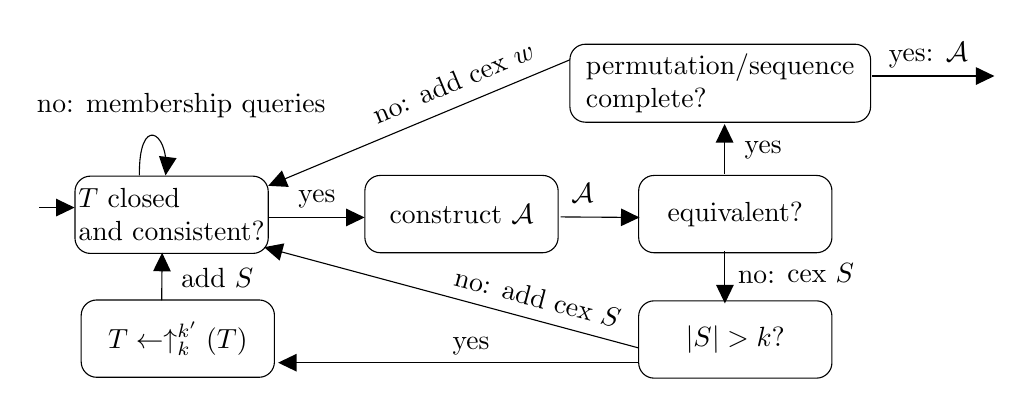
\begin{tikzpicture}[x=0.75pt,y=0.75pt,yscale=-1,xscale=1]
%uncomment if require: \path (0,427.3333320617676); %set diagram left start at 0, and has height of 427.3333320617676

%Curve Lines [id:da3242324591734014] 
\draw    (78.05,195.76) .. controls (77.68,166.57) and (91.81,174.17) .. (90.87,193.02) ;
\draw [shift={(90.63,195.76)}, rotate = 276.98] [fill={rgb, 255:red, 0; green, 0; blue, 0 }  ][line width=0.08]  [draw opacity=0] (8.93,-4.29) -- (0,0) -- (8.93,4.29) -- cycle    ;

%Rounded Rect [id:dp5230596682902247] 
\draw   (285.46,140.05) .. controls (285.46,135.9) and (288.82,132.53) .. (292.98,132.53) -- (422.81,132.53) .. controls (426.96,132.53) and (430.33,135.9) .. (430.33,140.05) -- (430.33,162.59) .. controls (430.33,166.74) and (426.96,170.11) .. (422.81,170.11) -- (292.98,170.11) .. controls (288.82,170.11) and (285.46,166.74) .. (285.46,162.59) -- cycle ;
%Straight Lines [id:da19996498797143802] 
\draw    (360,195) -- (360,174) ;
\draw [shift={(360,171)}, rotate = 450] [fill={rgb, 255:red, 0; green, 0; blue, 0 }  ][line width=0.08]  [draw opacity=0] (8.93,-4.29) -- (0,0) -- (8.93,4.29) -- cycle    ;

%Straight Lines [id:da7742261006504376] 
\draw    (360.15,232.33) -- (360.15,254.42) ;
\draw [shift={(360.15,257.42)}, rotate = 270] [fill={rgb, 255:red, 0; green, 0; blue, 0 }  ][line width=0.08]  [draw opacity=0] (8.93,-4.29) -- (0,0) -- (8.93,4.29) -- cycle    ;

%Straight Lines [id:da7240079665223356] 
\draw    (318.59,285.97) -- (147.88,285.97) ;
\draw [shift={(144.88,285.97)}, rotate = 360] [fill={rgb, 255:red, 0; green, 0; blue, 0 }  ][line width=0.08]  [draw opacity=0] (8.93,-4.29) -- (0,0) -- (8.93,4.29) -- cycle    ;

%Straight Lines [id:da4355292395155117] 
\draw    (88.79,255.9) -- (88.97,236) ;
\draw [shift={(89,233)}, rotate = 450.53] [fill={rgb, 255:red, 0; green, 0; blue, 0 }  ][line width=0.08]  [draw opacity=0] (8.93,-4.29) -- (0,0) -- (8.93,4.29) -- cycle    ;

%Straight Lines [id:da9395518765143251] 
\draw    (140,216) -- (183.56,216) ;
\draw [shift={(186.56,216)}, rotate = 180] [fill={rgb, 255:red, 0; green, 0; blue, 0 }  ][line width=0.08]  [draw opacity=0] (8.93,-4.29) -- (0,0) -- (8.93,4.29) -- cycle    ;

%Straight Lines [id:da9876991440040634] 
\draw    (280.98,215.74) -- (316,215.98) ;
\draw [shift={(319,216)}, rotate = 180.4] [fill={rgb, 255:red, 0; green, 0; blue, 0 }  ][line width=0.08]  [draw opacity=0] (8.93,-4.29) -- (0,0) -- (8.93,4.29) -- cycle    ;

%Straight Lines [id:da8894863053773812] 
\draw    (318.59,278.87) -- (141.02,231.11) ;
\draw [shift={(138.12,230.33)}, rotate = 375.05] [fill={rgb, 255:red, 0; green, 0; blue, 0 }  ][line width=0.08]  [draw opacity=0] (8.93,-4.29) -- (0,0) -- (8.93,4.29) -- cycle    ;

%Rounded Rect [id:dp7304454638728446] 
\draw   (318.59,203.21) .. controls (318.59,199.09) and (321.93,195.76) .. (326.04,195.76) -- (404.26,195.76) .. controls (408.37,195.76) and (411.71,199.09) .. (411.71,203.21) -- (411.71,225.56) .. controls (411.71,229.67) and (408.37,233) .. (404.26,233) -- (326.04,233) .. controls (321.93,233) and (318.59,229.67) .. (318.59,225.56) -- cycle ;
%Straight Lines [id:da989641097303189] 
\draw    (285.46,140.05) -- (142.89,199.6) ;
\draw [shift={(140.12,200.76)}, rotate = 337.33000000000004] [fill={rgb, 255:red, 0; green, 0; blue, 0 }  ][line width=0.08]  [draw opacity=0] (8.93,-4.29) -- (0,0) -- (8.93,4.29) -- cycle    ;

%Straight Lines [id:da5782151978812646] 
\draw    (431,147.86) -- (487,147.86) ;
\draw [shift={(490,147.86)}, rotate = 180] [fill={rgb, 255:red, 0; green, 0; blue, 0 }  ][line width=0.08]  [draw opacity=0] (8.93,-4.29) -- (0,0) -- (8.93,4.29) -- cycle    ;

%Rounded Rect [id:dp9174543196821443] 
\draw   (186.68,203.21) .. controls (186.68,199.09) and (190.02,195.76) .. (194.13,195.76) -- (272.35,195.76) .. controls (276.46,195.76) and (279.8,199.09) .. (279.8,203.21) -- (279.8,225.56) .. controls (279.8,229.67) and (276.46,233) .. (272.35,233) -- (194.13,233) .. controls (190.02,233) and (186.68,229.67) .. (186.68,225.56) -- cycle ;
%Rounded Rect [id:dp013423076978946291] 
\draw   (318.59,263.62) .. controls (318.59,259.51) and (321.93,256.17) .. (326.04,256.17) -- (404.26,256.17) .. controls (408.37,256.17) and (411.71,259.51) .. (411.71,263.62) -- (411.71,285.97) .. controls (411.71,290.08) and (408.37,293.42) .. (404.26,293.42) -- (326.04,293.42) .. controls (321.93,293.42) and (318.59,290.08) .. (318.59,285.97) -- cycle ;
%Rounded Rect [id:dp7630850927481354] 
\draw   (47.01,203.54) .. controls (47.01,199.42) and (50.35,196.09) .. (54.46,196.09) -- (132.68,196.09) .. controls (136.79,196.09) and (140.12,199.42) .. (140.12,203.54) -- (140.12,225.89) .. controls (140.12,230) and (136.79,233.33) .. (132.68,233.33) -- (54.46,233.33) .. controls (50.35,233.33) and (47.01,230) .. (47.01,225.89) -- cycle ;
%Rounded Rect [id:dp6612685395327704] 
\draw   (50,263.2) .. controls (50,259.09) and (53.34,255.76) .. (57.45,255.76) -- (135.67,255.76) .. controls (139.78,255.76) and (143.11,259.09) .. (143.11,263.2) -- (143.11,285.55) .. controls (143.11,289.66) and (139.78,293) .. (135.67,293) -- (57.45,293) .. controls (53.34,293) and (50,289.66) .. (50,285.55) -- cycle ;
%Straight Lines [id:da6707127407283302] 
\draw    (29.79,211.24) -- (43.84,211.24) ;
\draw [shift={(46.84,211.24)}, rotate = 180] [fill={rgb, 255:red, 0; green, 0; blue, 0 }  ][line width=0.08]  [draw opacity=0] (8.93,-4.29) -- (0,0) -- (8.93,4.29) -- cycle    ;


% Text Node
\draw (141.81,182.12) node   [align=left] {$ $};
% Text Node
\draw (93.57,214.71) node   [align=left] {$\displaystyle T${\fontfamily{ptm}\selectfont  }~closed \\and consistent?};
% Text Node
\draw (98.22,162.32) node   [align=left] {no: membership queries};
% Text Node
\draw (233.24,214.38) node   [align=left] {construct $\displaystyle \mathcal{A}$};
% Text Node
\draw (357.89,151.32) node   [align=left] {permutation/sequence \\complete?};
% Text Node
\draw (229.13,150.68) node  [rotate=-337.24] [align=left] {no: add cex~{\fontfamily{ptm}\selectfont  }$\displaystyle w$};
% Text Node
\draw (365.15,214.38) node   [align=left] {equivalent?};
% Text Node
\draw (394.44,242.91) node  [rotate=-359.45] [align=left] {no: cex $\displaystyle S$};
% Text Node
\draw (365.15,274.8) node  [rotate=-359.45] [align=left] {$\displaystyle |S| >k?$};
% Text Node
\draw (378.6,183.41) node  [rotate=-359.45] [align=left] {yes};
% Text Node
\draw (163.6,207.37) node  [rotate=-359.45] [align=left] {yes};
% Text Node
\draw (291.5,204) node   [align=left] {{\fontfamily{ptm}\selectfont  }$\displaystyle \mathcal{A}$};
% Text Node
\draw (269.92,254.66) node  [rotate=-14.77] [align=left] {no: add cex $\displaystyle S${\fontfamily{ptm}\selectfont  }};
% Text Node
\draw (237.84,277.89) node  [rotate=-359.61] [align=left] {yes};
% Text Node
\draw (458.14,137.71) node  [rotate=-359.45] [align=left] {yes: {\fontfamily{ptm}\selectfont  }$\displaystyle \mathcal{A}$};
% Text Node
\draw (115.57,245.15) node  [rotate=-359.61] [align=left] {add~{\fontfamily{ptm}\selectfont  }$\displaystyle S${\fontfamily{ptm}\selectfont  }};
% Text Node
\draw (96.56,274.38) node   [align=left] {{\fontfamily{ptm}\selectfont  }$\displaystyle T\leftarrow \uparrow ^{k'}_{k}( T)${\fontfamily{ptm}\selectfont  }};


\end{tikzpicture}
}

\caption{The learning process flow for $\nfhf$ and $\nfhe$.}
\label{fig:learning_flow}
\vspace{-3mm}
\end{figure}


